\documentclass[10pt]{report}
\usepackage[utf8]{inputenc}
%\usepackage[T1]{fontenc}
\usepackage{tgbonum}
\usepackage[english]{babel}
\usepackage{graphicx}
\usepackage{amsmath}
\usepackage{amssymb}
\usepackage{hyperref}
\usepackage{epsf}
\usepackage{float}
\usepackage{mathpazo}
\usepackage{pifont}
\usepackage
[
a4paper,% other options: a3paper, a5paper, etc
left=2.2cm,
right=2.2cm,
top=3cm,
bottom=3cm,
]{geometry}
%\geometry{hmargin=3.5cm, vmargin=2.5cm}
\usepackage{fancyhdr}
\pagestyle{fancy}
\fancyhf{}
\rfoot{\thepage}
\renewcommand{\headrulewidth}{0pt}
\usepackage{color}
\graphicspath{{DWGs/}}
\usepackage{graphicx}
\usepackage{wrapfig}
\usepackage{graphicx}
\usepackage{multicol}
\usepackage{enumitem}
\usepackage{xcolor}
\usepackage{framed}
\definecolor{shadecolor}{RGB}{139, 231, 3}
\usepackage{epigraph}

\usepackage{tcolorbox}
\definecolor{mycolor}{rgb}{0.122, 0.435, 0.698}

\newtcbox{\mb}{nobeforeafter,colframe=mycolor,colback=mycolor!10!white,boxrule=0.5pt,arc=4pt,
  boxsep=0pt,left=6pt,right=6pt,top=3pt,bottom=3pt,tcbox raise base}

\usepackage{eso-pic}
\newcommand\BackgroundPic{%
\put(-50,-0){%
\parbox[b][\paperheight]{\paperwidth}{%
\vfill
\centering
\includegraphics[height=\paperheight,%
keepaspectratio]{DWGs/cover.png}%
\vfill
}}}

\usepackage{emerald}
\usepackage[T1]{fontenc}

\usepackage{anyfontsize}
\usepackage{t1enc}
\newcommand{\heart}{\ensuremath\varheartsuit}
\usepackage{tikz}
\usetikzlibrary{positioning}

% CHAPTER STYLE =================================================

\makeatletter
\def\thickhrulefill{\leavevmode \leaders \hrule height 1ex \hfill \kern \z@}
\def\@makechapterhead#1{%
  \vspace*{10\p@}%
  {\parindent \z@ \raggedleft \reset@font
            \scshape \@chapapp{} \thechapter
        \par\nobreak
        \interlinepenalty\@M
    \Huge \bfseries #1\par\nobreak
    %\vspace*{1\p@}%
    %\hrulefill
    \par\nobreak
    \vskip 50\p@
  }}
\def\@makeschapterhead#1{%
  \vspace*{10\p@}%
  {\parindent \z@ \raggedleft \reset@font
            \scshape \vphantom{\@chapapp{} \thechapter}
        \par\nobreak
        \interlinepenalty\@M
    \Huge \bfseries #1\par\nobreak
    %\vspace*{1\p@}%
    %\hrulefill
    \par\nobreak
    \vskip 50\p@
  }}

\begin{document}

% TITLE PAGE ====================================================

\begin{titlepage}
\AddToShipoutPicture*{\BackgroundPic}
\ \\[4cm]
{\sffamily \color{white}
\begin{center}
\fontsize{66}{10}\selectfont \fontfamily{qcr}\selectfont Fluid  Toolbox

\vskip 10\p@

\fontsize{25}{10} \ECFAugie{with Python}

\end{center}
}
\vfill
{\fontsize{20}{20}\color{white}\sffamily Science Docs \hfill\color{white} Kamila Zdybał}
\end{titlepage}


% EX LIBRIS PAGE ================================================

\thispagestyle{empty}
\begin{center}
\vspace*{4cm}
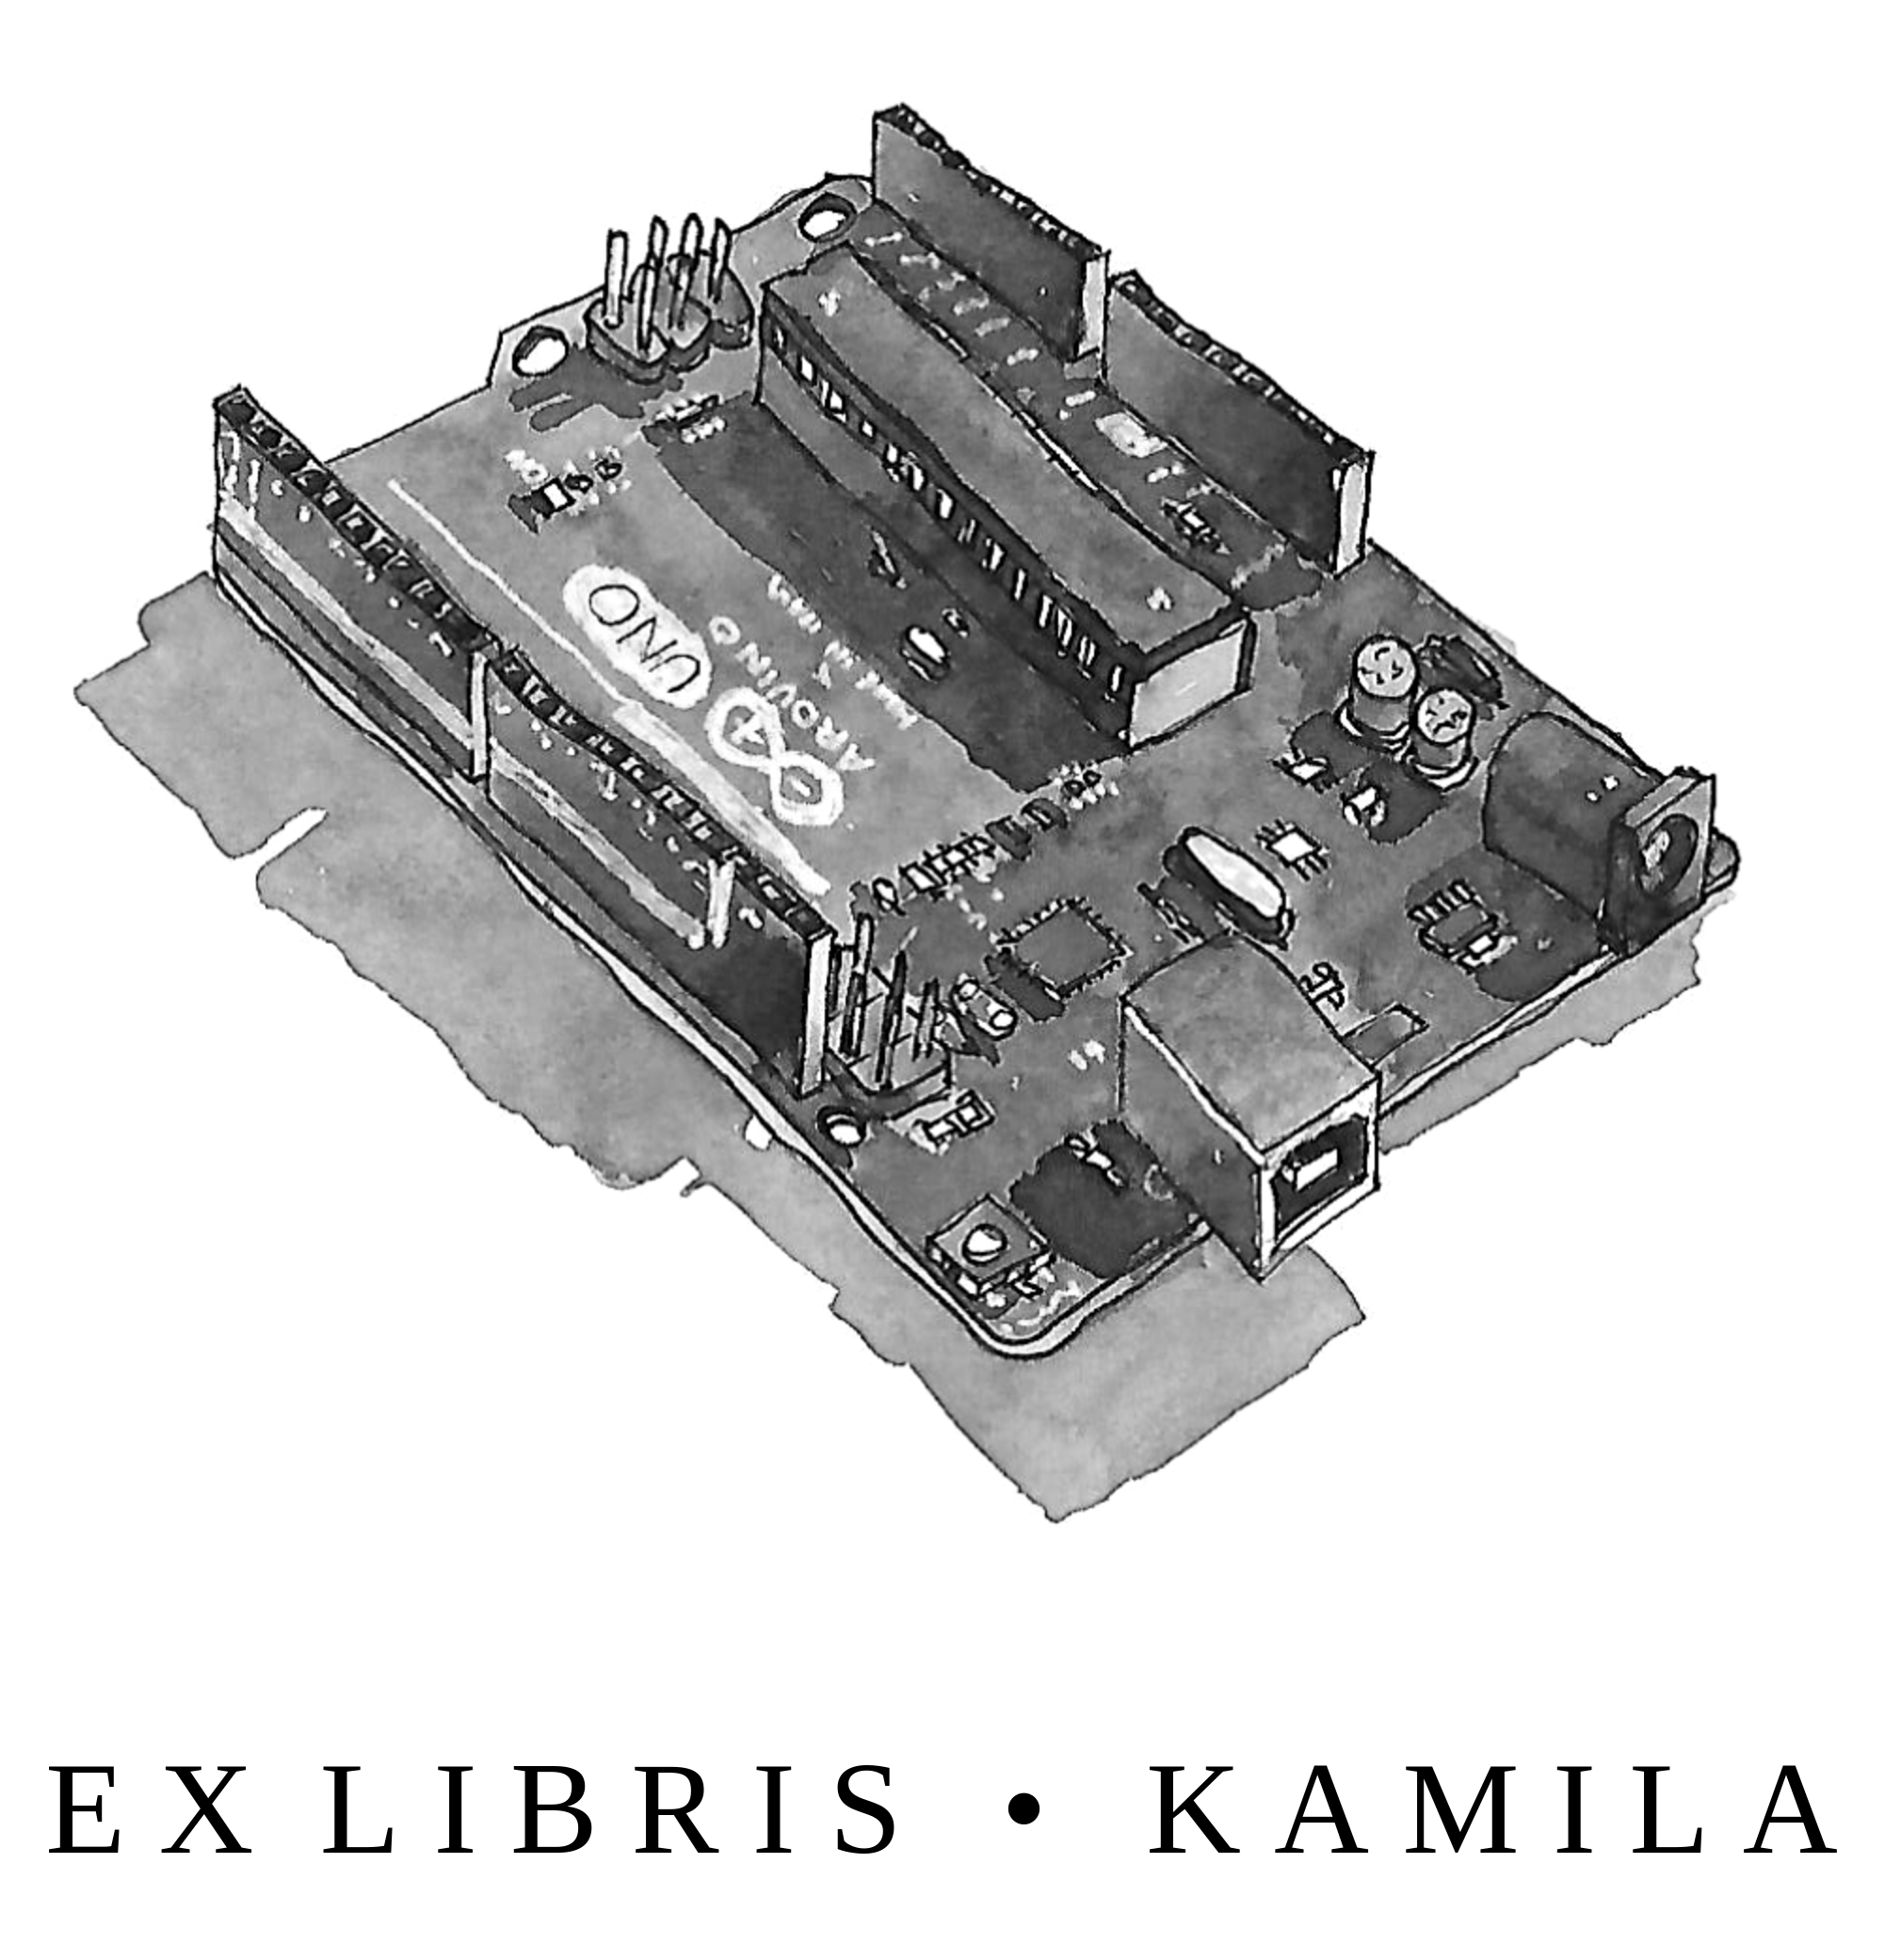
\includegraphics[width = 80mm]{ex_libris_arduino.png}

\vspace*{2cm}

Copyright \textcopyright \, K. Zdybał, 2018

For more projects similar to this one

visit me on GitHub: \verb|@camillejr|

\verb|camillejr.github.io/science-docs/|

To contact me personally drop me a line at:

\verb|kamilazdybal@gmail.com|

\vspace*{2cm}

\verb|Fluid Toolbox|

\verb|version 1.0|

Typeset with \ding{170} for \LaTeX

\vspace*{1.8cm}

\noindent This work is licensed under the Creative Commons

Attribution-NonCommercial-ShareAlike 4.0 International 

(CC BY-NC-SA
4.0) license.
\end{center}



\setlength{\parskip}{0.6em}
\setlength{\parindent}{0cm}

\tableofcontents

\chapter*{Preface}
\chaptermark{Preface}
% Fluid Toolbox content

\rightline{{\rm \textit{"Use it well."}}}

\rightline{{\rm --- Prof. Albus Dumbledore}}

\textbf{Fluid Toolbox \ECFAugie{with Python}} is a collection of human-readable, pseudo-random study notes. It contains descriptions and explanations of fluid mechanics concepts, presented in a way that resembles the record of my understanding of them. It is meant to be used complimentary to the regular textbook, since it may provide additional insight but it will not substitute thoroughness of a standard course in the subject. I believe that working side by side with a course it can become indeed a useful toolbox of concepts that are ready-to-understand and read-to-use.

These notes are under constant development as I learn more and understand more.

\section*{Why is this text created?}

I have a goal of laying the ground for the most important fluid mechanics concept and collecting them in once place. Much of the knowledge presented here comes from my searching of understanding that I was often missing when reading textbooks, and which was difficult to find in a way that would be pleasant and intuitive. Much of the understanding presented here comes from my personal explorations and thinking on the subject and therefore I have hopes that Fluid Toolbox will become a helpful resource that you have been looking for, similarly as it would have been helpful when I was looking for similar set of notes.

\section*{Structure of the text}

Each concept is presented as a separate chapter.

\section*{A note of inspiration and motivation}




\chapter{Changes}

Changes are modeled by derivatives. Derivative explains how much one variable $\phi_1$ change when we change the other $\phi_2$, and we express this in mathematical terms:

\begin{equation}\label{eq:change-d}
\frac{d \phi_1}{d \phi_2}
\end{equation}

where the letter $d$ stands for \textit{the change of...} and is later followed by the variable that we are speaking of. So really the above ratio means: there is this much change of variable $\phi_1$ per this much change of variable $\phi_2$. In fluid dynamics, you will find that we are most interested with two types of changes: change in time and change in space (position). Therefore you will most often encounter $dt$ or $dx$, $dy$, $dz$ in the denominator of various forms of Eq. (\ref{eq:change-d}). Since we live in the three-dimensional space with a time arrow, it is justifiable why these two have the biggest popularity, right?

There is also another mathematical expression for a derivative and it is:

\begin{equation}\label{eq:change-partial}
\frac{\partial \phi_1}{\partial \phi_2}
\end{equation}

The operator $\partial$ (called "partial" or "del") also stands for \textit{the change of...} but it also give you a hint that the variable $\phi_1$ can change with a change of variables other than $\phi_2$. Perhaps it can also change with some $\phi_3$ and $\phi_4$, even though in this particular ratio from Eq. (\ref{eq:change-partial}) we are only interested in a change with $\phi_2$.

\section{What does it mean for a quantity to change in time and in space?}


\subsection{Steady-state case and a time derivative}

\section{Convention for the sign of a derivative}

For the purpose of this demonstration we will look at the derivative $\frac{dp}{dx}$ - change in pressure per change in the $x$-axis position - which is often encountered in fluid dynamics. We will lay the ground for what does it mean for this derivative to be positive, negative or zero, and why the reasoning makes sense.

Suppose that the initial point is marked with \textcolor{myblue}{$(i)$} and it is always a point at coordinate $x$. The point to which we move after one space-step, the final point, is marked with \textcolor{myblue}{$(f)$} and is either at $x+dx$ or $x - dx$ coordinate, depending on the positive or negative change that we decide to make. The direction of the change on the $x$-axis is marked with a blue arrow.

\begin{figure}[H]
\begin{subfigure}[t]{.46\textwidth}
\centering
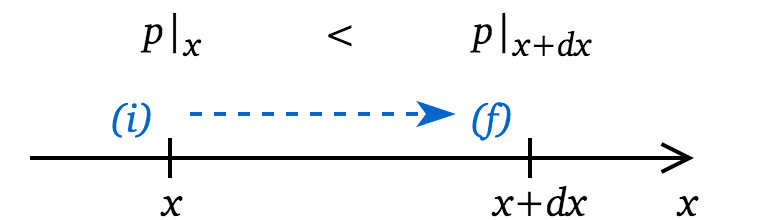
\includegraphics[scale=.2]{dp-dx-pos-neg.png}
\caption{$\frac{dp}{dx} > 0$ with positive change in $x$.}
\end{subfigure}
\begin{minipage}[t]{.07\textwidth}
$ $
\vspace*{1.5cm}
\end{minipage}
\begin{subfigure}[t]{.46\textwidth}
\centering
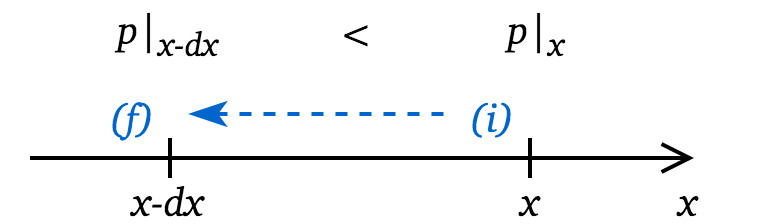
\includegraphics[scale=.2]{dp-dx-neg-neg.png}
\caption{$\frac{dp}{dx} > 0$ with negative change in $x$.}
\end{subfigure}
\begin{subfigure}[t]{.46\textwidth}
\centering
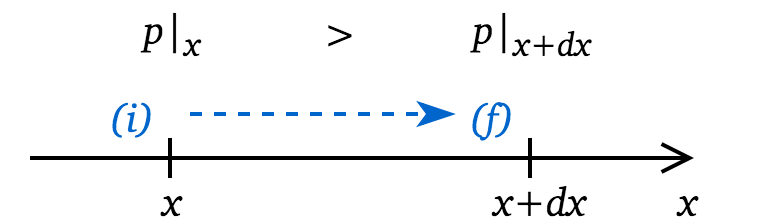
\includegraphics[scale=.2]{dp-dx-pos-pos.png}
\caption{$\frac{dp}{dx} < 0$ with positive change in $x$.}
\end{subfigure}
\begin{minipage}[t]{.08\textwidth}
$ $
\end{minipage}
\begin{subfigure}[t]{.46\textwidth}
\centering
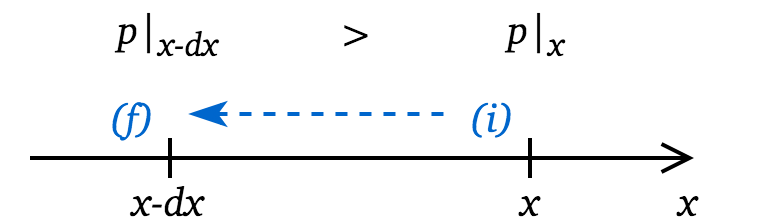
\includegraphics[scale=.2]{dp-dx-neg-pos.png}
\caption{$\frac{dp}{dx} < 0$ with negative change in $x$. }
\end{subfigure}
\caption{Sign of the $\frac{dp}{dx}$ derivative versus directions of the change along the $x$-axis.}
\label{fig:dp-dx-signs}
\end{figure}

We will now find out for all cases which pressure, at \textcolor{myblue}{$(i)$} or at \textcolor{myblue}{$(f)$} must be larger. Our aim is to show that situations (a) and (b) in Figure \ref{fig:dp-dx-signs} must be equivalent - they explain the same physical phenomena. In both of these cases we will show that the pressure is increasing with the increasing $x$-coordinate, independent of whether we decide to take a step to the right or to the left of our initial point \textcolor{myblue}{$(i)$}. 

We will show the analogical result can be said about situations (c) and (d) but in this case the pressure is decreasing with the increasing $x$-coordinate.



\subsection{Closing note}

The analysis done in this section is often necessary in order to find out whether or not to "put a minus sign" in front of the equations. For instance, as we will show later in the text, such reasoning can help us understand why there is a minus sign in the Euler equation for a fluid element experiencing pressure force: $dp = - \rho \upsilon d \upsilon$. Oftentimes, the sign of a derivative tells an important information about the nature of the physical phenomena.








\chapter{Differentiation}

Differentiation is a way to make discrete things continuous.

\chapter{Common flow types}

\section{Signs convention for fluid elements}

A fluid laminate with a lower $y$-coordinate exerts force on a fluid laminate with a bigger $y$-coordinate. With Newton's 3rd law we can therefore state that a fluid laminate with a bigger $y$-coorinate exerts negative force on a fluid laminate with a lower $y$-coordinate.

Similarly in the $x$-direction, a fluid element with a lower $x$-coordinate exerts force on a fluid element with a bigger $x$-coordinate and taking Newton's 3rd law, a fluid element with a bigger $x$-coordinate exerts negative force on a fluid element with a lower $x$-coordinate

\section{Newtonian fluids}



\section{Poiseuille flow}

Consider a steady-state flow of fluid between two parallel plates. We would like to find the velocity and shear stress distribution along the $y$-axis.The pressure drop is assumed to be constant throughout the channel. This means that the pressure is a function of position $p = p(x)$ but the change in pressure per every equal distance in the channel is constant: $dp/dx = \text{const}$. The width of the channel $B$ is much larger compared to its other dimensions.

\begin{figure}[H]
\centering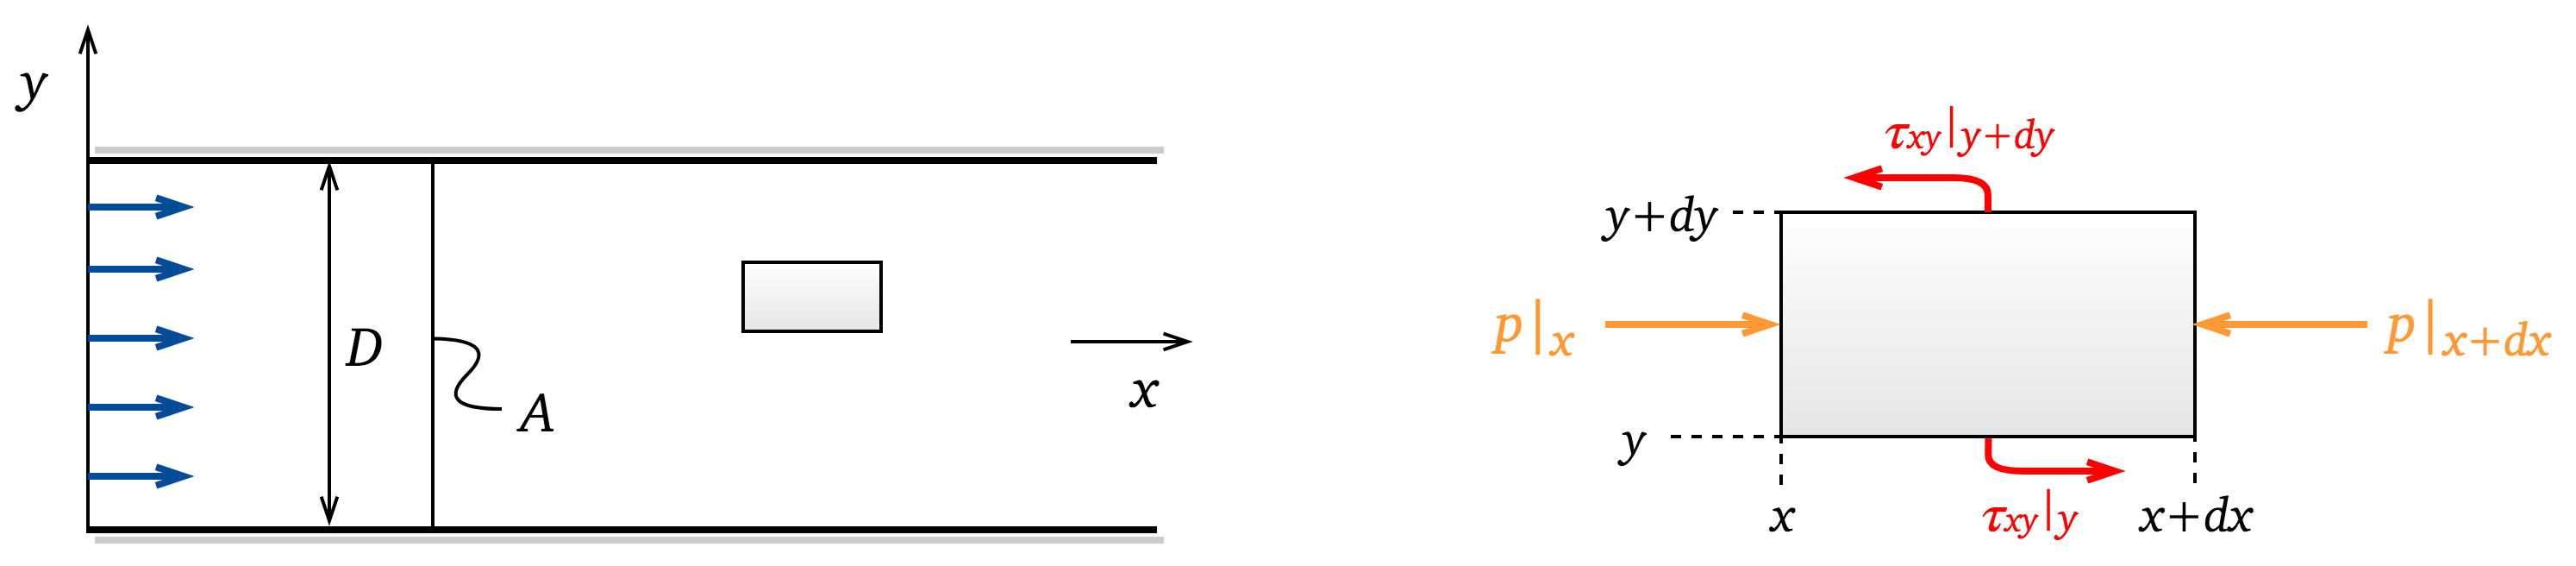
\includegraphics[width=15cm]{poiseuille-fluid-element}
\caption{Flow between two parallel plates with an infinitesimal fluid element.}			
\label{fig:poiseuille-fluid-element}
\end{figure}

We also have three boundary conditions. Due to a no-slip condition we assume that the velocity at the very surface of the plates is zero: $u(-D/2) = 0$ and $u(D/2) = 0$. Due to symmetry of the flow we assume that there cannot be any net momentum transfer between the upper half and the lower half of the channel. Hence, the shear stress exactly in the middle of the channel is zero: $\tau_{xy}(0) = 0$.

Steady state momentum (force) balance, taking into account pressure and shear forces on a single infinitesimal fluid element:

\begin{equation}
0 = p|_x B dy - p|_{x+dx} B dy + \tau_{xy}|_y B dx - \tau_{yx}|_{y+dy} B dx
\end{equation}

Dividing both sides by the width $B$ and by $dx dy$ we obtain:

\begin{equation}
0 = \frac{p|_x  - p|_{x+dx}}{dx}  + \frac{\tau_{xy}|_y  - \tau_{yx}|_{y+dy}}{dy} 
\end{equation}

Now we notice that $\frac{p|_x  - p|_{x+dx}}{dx}$ is in fact equal to $-\frac{dp}{dx}$ (in a limit as $dx \rightarrow 0$), since it is an incremental change in pressure function value per incremental distance $dx$. Similar thing can be said about $\frac{\tau_{xy}|_y  - \tau_{yx}|_{y+dy}}{dy}$ which is equal to $-\frac{d \tau_{xy}}{dy}$. We can thus further simplify:

\begin{equation}
\frac{d \tau_{xy}}{dy} = - \frac{dp}{dx} = \text{const}
\end{equation}

Integrating the above equation and applying the initial condition for the shear stress $\tau_{xy}(0) = 0$:

\begin{equation} \label{eq:shear-poiseuille}
\tau_{xy}(y)= - \frac{dp}{dx} y
\end{equation}

Adding a constitutive relation for Newtonian fluids we can further relate pressure and velocity. From the Newton's law we know also that:

\begin{equation} \label{eq:shear-newton}
\tau_{xy}(y)= - \mu \frac{du}{dy}
\end{equation}

You may look at this in such a way: the equation \ref{eq:shear-poiseuille} is a special case in which the shear stresses have been related to the driving force in the Poiseuille flow - the pressure gradient. The equation \ref{eq:shear-newton} is a general description of any shear stress $\tau_{xy}$, where it is linked to velocity gradients, no matter what the cause for this velocity gradient is! It just so happens that in the case of a Poiseuille flow between two parallel plates this cause is the pressure drop:

\begin{equation}
- \mu \frac{du}{dy} = - \frac{dp}{dx} y
\end{equation}

Integrating one more time the above relation and applying the no-slip boundary conditions we get:

\begin{equation}
u(y) = \frac{1}{2 \mu} \frac{dp}{dx} (y^2 - (D/2)^2)
\end{equation}





\chapter{Drag force}

The mathematical description of the drag force begins with making a guess. It is an intuitive guess which answers the question: what physical quantities affect the value of the drag force on an object moving through a fluid? The thought process done on this question gives the following four quantities:

relative fluid-object velocity $\upsilon$ \,\,\,\,\,\,\,\,\,\,\,\,\,\,\,  fluid density $\rho$ \,\,\,\,\,\,\,\,\,\,\,\,\,\,\, fluid viscosity $\mu$ \,\,\,\,\,\,\,\,\,\,\,\,\,\,\, geometry of an object $D$

We assume that the drag force is a combination of these quantities to some yet unknown powers and we use dimensional analysis to find those powers.

\begin{equation}
F_D = \upsilon^a \rho^b \mu^c D^d
\label{eq:drag_force}
\end{equation}

Writing out the units of the above equation we get:

\begin{equation*}
\Big[ \frac{kg \cdot m}{s^2} \Big] = \Big[ \frac{m}{s} \Big]^a \cdot \Big[ \frac{kg}{m^3} \Big]^b \cdot \Big[ \frac{kg}{m \cdot s} \Big]^c \cdot \Big[ m \Big]^d
\end{equation*}

Shuffling around a bit:

\begin{equation*}
kg \cdot m \cdot s^{-2} = kg^{b+c} \cdot m^{a -3b - c + d} \cdot s^{-a - c}
\end{equation*}

Hence:

$1 = b+c$

$1 = a - 3b - c + d$

$-2 = - a - c$

The simple fact that this set of equations cannot be solved exactly (there is four  uknown powers and only three equations) is going to call experiment for help, which you will notice in the next few passages.

Let's then write the set of equations by means of one of the unknowns $c$:

$a = 2 - c$

$b = 1 - c$

$d = 2 - c$

\newpage

Subsituting back to the equation \ref{eq:drag_force} we get:

\begin{equation}
F_D = \upsilon^{2 - c} \rho^{1 - c} \mu^c D^{2 - c} 
\label{eq:drag_force_powers}
\end{equation}

Structuring the equation still a bit gives:

\begin{equation}
F_D = \upsilon^2 \rho D^2 \cdot \Big[ \frac{\upsilon \rho D}{\mu} \Big]^{-c}
\label{eq:drag_force_powers}
\end{equation}

It always feels comfortable to find the Reynolds number in your equation, so there it is:

\begin{equation}
F_D = \upsilon^2 \rho D^2 Re^{-c}
\label{eq:drag_force_powers}
\end{equation}

We get finally that the drag force is proportional to some unknown power of the Reynolds number.


In fact, we will not leave it there yet, since there is an interesting last point to say. Instead of the above equation, we will say that the drag force is proportional to some unknown function $C_D$ of the Reynolds number. We also recognise that we may rewrite the quantity $\upsilon^2 \rho$ as the dynamic pressure $\frac{\upsilon^2 \rho}{2}$, since multiplying the right hand side by $\frac{1}{2}$ will not spoil the dimensional equality of both sides. The quantity $D^2$ has got the unit of area, so we exchange it for the quantity $A_{\perp}$, representing the frontal area of an object. The equation for the drag force becomes:

\begin{equation}
F_D = \frac{\upsilon^2 \rho}{2} A_{\perp} C_D (Re)
\label{eq:drag_force_powers}
\end{equation}

The unknown function $C_D (Re)$ is called the \textbf{drag coefficient}. That is where we call for experiment.

Questions:

What would have happened if we wrote the powers in terms of some power other than $c$?












\chapter{Circulation}



Circulation is defined as:

\begin{equation}
\Gamma = \oint_C \vec{\upsilon} \cdot \vec{dl}
\end{equation}

The dot operation gives a scalar which is expressing "how much" in the direction of the other vector is this vector.

\begin{figure}[H]
\centering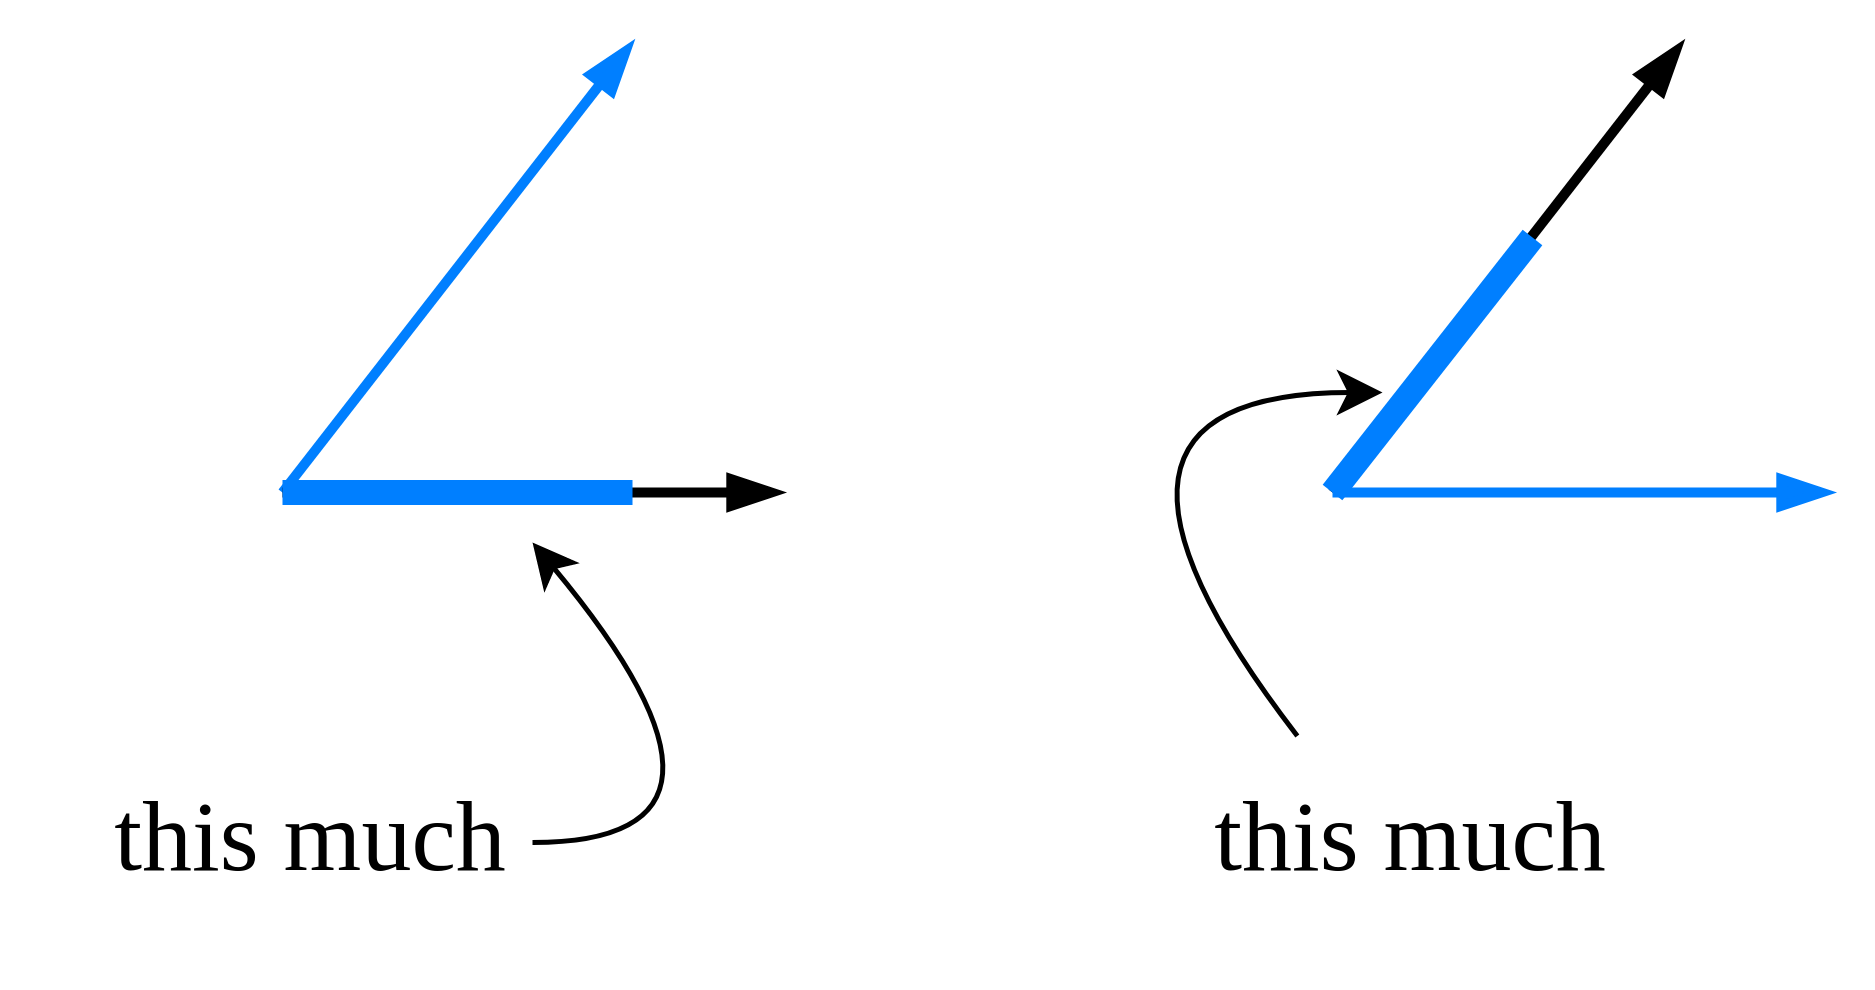
\includegraphics[width=5cm]{circulation_dot_prod}
\caption{Dot product of two vectors.}			
\label{fig:learning_curve}
\end{figure}

When they are $\perp$, the dot product is zero.

In the concept of circulation, you ask "how much" at any point on the curve $C$ the velocity vector at that point is in the direction of the curve's geometry. Now, that doesn't yet sound as something to do with "circulating". For the moment, I would think that it's more of an "on-trackness". Something, that in real world would be for instance the measure of how much the vehicle's velocity is in the direction of the road geometry.

But then you realise an important detail of "$\circ$" on the integral symbol, which means that the curve should be a closed curve - a loop.

When you perform integration, which means summing up every little $\vec{\upsilon} \cdot \vec{dl}$ as you go around the loop, you count "how much" at every point on the loop, the velocity vector at these points is in the direction of the loop's geometry (at these points).

If we were to place a small particle at some starting point $P$ on the loop, the circulation would tell us "how much" the velocity field which this particle is subjected to, is tending to move that particle around the loop.

It can be very intuitive when you take a look at these two pictures:



It's no surprise that when the velocity is everywhere perpendicular to the loop's geometry, the circulation around the loop is zero. If you were to place a particle at any point on the loop, such velocity field would act to immediately displace the particle off the loop. Therefore, the particle would have no way of "circulating" around the loop.

On the other extreme is the case when the velocity field is everywhere tangent to the loop's geometry. Anywhere the particle goes on the loop, the velocity at that point would act to keep the particle moving around the loop.

Questions:

\begin{enumerate}
\item Why closed loop? Would it have any meaning if we calculated circulation along any general spline?

\item How to chose loops so that the circulation we calculate is of the most meaning to us?

\item What does the zero, positive, negative circulation mean?

\item Can circulation be infinite?
\end{enumerate}



\chapter{Vorticity}


\begin{enumerate}
\item Why is vorticity concept needed? Isn't it something kind of like circulation?

\end{enumerate}


\chapter{Stoke's theorem}






\chapter{Nondimensionalizing}


What's with the nondimensionalizing? 

\chapter{Material derivative}

\chapter{Conservation of mass}

In this chapter we present the derivation of the conservation of mass equation, otherwise known as the \textbf{continuity equation}. In principle, it states that mass cannot be lost nor created.

We begin by writing out the overall mass balance inside any control volume CV. The net change of mass inside the control volume is equal to the mass flowing into the CV minus the mass flowing out of the CV. Note here, that when the net change of mass in a CV is not zero (unsteady case), it can only be due to either compression (more mass flowing in than flowing out) or decompression (more mass flowing out than flowing in). The general mass balance is:

\begin{equation} \label{eq:net_change}
\text{net change} = \text{flow in} - \text{flow out}
\end{equation}

\section{Mass flow rate}

\section{Derivation}

We are going to write out the RHS of the equation \ref{eq:net_change} as the difference between mass flow rate in and mass flow rate out in three Cartesian directions.

In the $x$-direction:

\begin{equation}
\Big( \rho u - \frac{\partial (\rho u)}{\partial x} \frac{dx}{2} \Big) dy dz - \Big( \rho u + \frac{\partial (\rho u)}{\partial x} \frac{dx}{2} \Big) dy dz = - \frac{\partial (\rho u)}{\partial x} dx dy dz
\end{equation}

In the $y$-direction:

\begin{equation}
\Big( \rho v - \frac{\partial (\rho v)}{\partial y} \frac{dy}{2} \Big) dx dz - \Big( \rho v + \frac{\partial (\rho v)}{\partial y} \frac{dy}{2} \Big) dx dz = - \frac{\partial (\rho v)}{\partial y} dy dx dz
\end{equation}

In the $z$-direction:

\begin{equation}
\Big( \rho w - \frac{\partial (\rho w)}{\partial z} \frac{dz}{2} \Big) dx dy - \Big( \rho w + \frac{\partial (\rho w)}{\partial z} \frac{dz}{2} \Big) dx dy = - \frac{\partial (\rho w)}{\partial z} dz dx dy
\end{equation}

The net change in time of mass can be written as:

\begin{equation}
\frac{\partial \rho}{dt} dx dy dz
\end{equation}

Putting all the terms together into equation \ref{eq:net_change} we obtain:

\begin{equation}
\frac{\partial \rho}{dt} dx dy dz = - \frac{\partial (\rho u)}{\partial x} dx dy dz - \frac{\partial (\rho v)}{\partial y} dy dx dz - \frac{\partial (\rho w)}{\partial z} dz dx dy
\end{equation}

Dividing both sides by $dx dy dz$ we get:

\begin{equation} \label{eq:continuity_general}
\frac{\partial \rho}{dt} = - \frac{\partial (\rho u)}{\partial x} - \frac{\partial (\rho v)}{\partial y} - \frac{\partial (\rho w)}{\partial z}
\end{equation}

Lastly, we can observe that the divergence of the quantity $\rho \vec{V}$ is:

\begin{equation}
\nabla (\rho \vec{V}) = \nabla (\rho \langle u, v, w \rangle) = \nabla \langle \rho u, \rho v, \rho w \rangle = \frac{\partial (\rho u)}{\partial x} + \frac{\partial (\rho v)}{\partial y} + \frac{\partial (\rho w)}{\partial z}
\end{equation}

So in the end, we can further write the RHS of the equation \ref{eq:continuity_general} in a shorter format as:

\begin{equation} \label{eq:continuity_divergence}
\frac{\partial \rho}{dt} = - \nabla (\rho \vec{V})
\end{equation}

\section{Special cases of density function}

In the most general case, the density $\rho$ is a function of time and space $\rho = \rho(t, x, y, z)$ and the equation \ref{eq:continuity_divergence} is written out for the most general case. Special cases can be defined when certain restrictions are imposed on the density function.

\subsection{Steady flow}

First, when the density $\rho$ is only a function of position $\rho = \rho(x,y,z)$ and does not change in time at any point in the flow field, we arrive at the steady state condition where the derivative $\frac{\partial \rho}{dt} = 0$.

The continuity equation then becomes:

\begin{equation} \label{eq:continuity_stst}
0 = - \rho \nabla \vec{V}
\end{equation}

\subsection{Incompressible flow}

When we assume that the density is constant in space, it can be taken out front of the divergence operator and the incompressible continuity equation is:

\begin{equation} \label{eq:continuity_incompressible}
\frac{\partial \rho}{dt} = - \rho \nabla \vec{V}
\end{equation}

The above equation corresponds to the density that is constant throughout the flow field at any moment in time, but can change in time in the entire flow field.

\subsection{Steady and incompressible flow}

The steady flow can be further combined with the incompressible condition, which disables the density to change both in time and space. The stead-state incompressible continuity equation then becomes:

\begin{equation} \label{eq:continuity_stst_incompressible}
0 = \nabla \vec{V}
\end{equation}

or writing the above equation with the use of partial differentiation operator:

\begin{equation}
\frac{\partial u}{\partial x} + \frac{\partial v}{\partial y} + \frac{\partial w}{\partial z} = 0
\end{equation}

\section{Dimension reduction}



\chapter{Gauss's law}

\chapter{Reynolds number}

\chapter{Constitutive equations}

\chapter{The Navier-Stokes equations}

The Navier-Stokes equations represent the momentum balance on an infinitesimal fluid volume. They state that the sum of forces acting on a fluid volume is equal to the change in momentum for that volume (Newton's second law).

\section{Incompressible Navier-Stokes}

In a three-dimensional, incompressible, unsteady flow we have:

$x$-direction:

\begin{equation} \label{eq:NS_x}
\rho g_x - \frac{\partial P}{\partial x} + \mu \Big( \frac{\partial^2 u}{\partial x^2} + \frac{\partial^2 u}{\partial y^2} + \frac{\partial^2 u}{\partial z^2}\Big) = \rho \Big( \frac{\partial u}{\partial t} + u \frac{\partial u}{\partial x} + v \frac{\partial u}{\partial y} + w \frac{\partial u}{\partial z} \Big)
\end{equation}

$y$-direction:

\begin{equation} \label{eq:NS_y}
\rho g_y - \frac{\partial P}{\partial y} + \mu \Big( \frac{\partial^2 v}{\partial x^2} + \frac{\partial^2 v}{\partial y^2} + \frac{\partial^2 v}{\partial z^2}\Big) = \rho \Big( \frac{\partial v}{\partial t} + u \frac{\partial v}{\partial x} + v \frac{\partial v}{\partial y} + w \frac{\partial v}{\partial z} \Big)
\end{equation}

$z$-direction:

\begin{equation} \label{eq:NS_z}
\rho g_z - \frac{\partial P}{\partial z} + \mu \Big( \frac{\partial^2 w}{\partial x^2} + \frac{\partial^2 w}{\partial y^2} + \frac{\partial^2 w}{\partial z^2}\Big) = \rho \Big( \frac{\partial w}{\partial t} + u \frac{\partial w}{\partial x} + v \frac{\partial w}{\partial y} + w \frac{\partial w}{\partial z} \Big)
\end{equation}

\section{Derivation}

Sum of the forces is written on the LHS of the above equations. The total change in momentum is written on the RHS of the above equations.

\subsection{RHS}

In the most general case, the velocity vector $\vec{V} = \langle u, v, w \rangle$ is a function of time and position. We write therefore: $\vec{V}(t, x, y, z) = \langle u(t, x, y, z), v(t, x, y, z), w(t, x, y, z) \rangle $.

The acceleration component is described as the time derivative of the corresponding velocity component. If you were to take the derivative with respect to time of any of the above components of the velocity vector, it would become due to chain rule:

\begin{equation}
a_x = \frac{\partial u(t,x,y,z)}{\partial t} = \frac{\partial u}{\partial t} \frac{\partial t}{\partial t} + \frac{\partial u}{\partial x} \frac{\partial x}{\partial t} + \frac{\partial u}{\partial y} \frac{\partial y}{\partial t} + \frac{\partial u}{\partial z} \frac{\partial z}{\partial t}
\end{equation}

Observe then, that $\frac{\partial t}{\partial t} = 1$, $\frac{\partial x}{\partial t} = u$, $\frac{\partial y}{\partial t} = v$, $\frac{\partial z}{\partial t} = w$.

We have therefore for all three components:

\begin{equation}
a_x = \frac{\partial u(t,x,y,z)}{\partial t} = \frac{\partial u}{\partial t} + u \frac{\partial u}{\partial x} + v \frac{\partial u}{\partial y} + w \frac{\partial u}{\partial z}
\end{equation}

\begin{equation}
a_y = \frac{\partial v(t,x,y,z)}{\partial t} = \frac{\partial v}{\partial t} + u \frac{\partial v}{\partial x} + v \frac{\partial v}{\partial y} + w \frac{\partial v}{\partial z}
\end{equation}

\begin{equation}
a_z = \frac{\partial w(t,x,y,z)}{\partial t} = \frac{\partial w}{\partial t} + u \frac{\partial w}{\partial x} + v \frac{\partial w}{\partial y} + w \frac{\partial w}{\partial z}
\end{equation}

The terms $\frac{\partial u}{\partial t}$, $\frac{\partial v}{\partial t}$, $\frac{\partial w}{\partial t}$ are called \textbf{local accelerations}, and the remaining terms where the derivatives are taken with respect to spacial coordinates are called \textbf{convective accelerations}\footnote{See the chapter on Material Derivative for more understanding of the local and convective terms.}. The names \textit{local} and \textit{convective} carry a lot of meaning here, although initially it might be hard to see. 

The word \textit{convective} means that it is a quantity that depends on traveling to other regions - in other words - it depends on position. It is going to change due to the fact that the fluid element has traveled to a new place.

The word \textit{local}, on the other hand, suggests that it is a quantity that is intrinsic to the particular fluid element and its change is independent of the particle's position in space. The \textit{local} quantity can change in a fluid element, but solely "in itself" as the time pass (or \textit{locally} and that will happen independent of where the fluid particle travels to). 

Notice that this logic fits into how these derivatives look like. The convective terms are all derivatives with respect to position - they account for a change in velocity components due to change in coordinates. The local terms are all derivatives with respect to time - they just change by itself as the time change and position is irrelevant.

The above equations represent the acceleration components. These components are present in the RHS of the Navier-Stokes equations [\ref{eq:NS_x} - \ref{eq:NS_z}].

The standard way to write the Newton's second law is that the sum of the forces equals mass multiplied by acceleration. Since the Navier-Stokes equations are written per volume basis, the change in momentum (or the mass multiplied by acceleration) is written per unit of volume, so:

\begin{equation}
\frac{dm}{dV} a_x = \frac{dm}{dV} \frac{\partial u(t,x,y,z)}{\partial t} = \rho \frac{\partial u(t,x,y,z)}{\partial t}
\end{equation}

Multiplying all the acceleration components by the density $\rho$ we are going to obtain the full description for the change in momentum per unit of volume:

\begin{equation}
\rho a_x = \rho \frac{\partial u(t,x,y,z)}{\partial t} = \rho \frac{\partial u}{\partial t} + \rho  u \frac{\partial u}{\partial x} + \rho v \frac{\partial u}{\partial y} + \rho w \frac{\partial u}{\partial z}
\end{equation}

\begin{equation}
\rho a_y = \rho \frac{\partial v(t,x,y,z)}{\partial t} = \rho \frac{\partial v}{\partial t} + \rho u \frac{\partial v}{\partial x} + \rho v \frac{\partial v}{\partial y} + \rho w \frac{\partial v}{\partial z}
\end{equation}

\begin{equation}
\rho a_z = \rho \frac{\partial w(t,x,y,z)}{\partial t} = \rho \frac{\partial w}{\partial t} + \rho u \frac{\partial w}{\partial x} + \rho v \frac{\partial w}{\partial y} + \rho w \frac{\partial w}{\partial z}
\end{equation}

This concludes the derivation and explanation of the RHS of the Navier-Stokes equations stated at the beginning of this chapter.


\subsection{LHS}

We are now going to crunch the LHS of the Navier-Stokes equations - the sum of the forces acting on a unit volume of fluid. There are two types of forces taken into account here: \textbf{body forces} (gravity) and \textbf{surface forces} (forces due to pressure difference and dissipative forces due to viscosity).

\subsubsection{Gravity forces}

The body forces due to gravity are perhaps the most intuitive to figure out. In order to construct the gravity force $F_{g, x}$ on a fluid element, we multiply mass of that element by gravitational acceleration. Inside the Navier-Stokes equations it is not any different. We have the terms: $\rho g_x$, $\rho g_y$, $\rho g_z$, that represent exactly that idea, except they are again written on a per volume basis.

\begin{equation}
\frac{d F_{g, x}}{dV} = \frac{dm}{dV} g_x =  \rho g_x
\end{equation}

\begin{equation}
\frac{d F_{g, y}}{dV} = \frac{dm}{dV} g_y =  \rho g_y
\end{equation}

\begin{equation}
\frac{d F_{g, z}}{dV} = \frac{dm}{dV} g_z =  \rho g_z
\end{equation}

\subsubsection{Surface forces}

The surface stresses can be represented by the stress tensor:

\begin{equation}
\bm{\sigma}_{IN} = \left(
\begin{matrix} 
\sigma_{xx} & \sigma_{xy} & \sigma_{xz} \\
\sigma_{yx} & \sigma_{yy} & \sigma_{yz} \\
\sigma_{zx} & \sigma_{zy} & \sigma_{zz}
\end{matrix}
\right)
\end{equation}

\begin{equation}
\bm{\sigma}_{OUT} = \left(
\begin{matrix} 
\sigma_{xx} + \frac{\partial \sigma_{xx}}{\partial x}dx & \sigma_{xy} + \frac{\partial \sigma_{xy}}{\partial y}dy & \sigma_{xz} + \frac{\partial \sigma_{xz}}{\partial z}dz \\
\sigma_{yx} + \frac{\partial \sigma_{yx}}{\partial x}dx & \sigma_{yy} + \frac{\partial \sigma_{yy}}{\partial y}dy & \sigma_{yz} + \frac{\partial \sigma_{yz}}{\partial z}dz \\
\sigma_{zx} + \frac{\partial \sigma_{zx}}{\partial x}dx & \sigma_{zy} + \frac{\partial \sigma_{zy}}{\partial y}dy & \sigma_{zz} + \frac{\partial \sigma_{zz}}{\partial z}dz 
\end{matrix}
\right)
\end{equation}

The net force on the fluid element resulting from the surface stresses

Writing out the :

$\sigma_{xx} dy dz$


$\sigma_{xx} dy dz - \frac{\partial \sigma_{xx}}{\partial x}$ 



In the $x$-direction: 

$\frac{\partial \sigma_{xx}}{\partial x}$ 

In the $y$-direction: 



In the $z$-direction: 









\section{Assumptions and limitations}






\begin{tikzpicture}
  \node[minimum height=0.8cm,minimum width=16.5cm, fill=lightgray,fill opacity=0.5,rounded
      corners=1ex,font=\fontsize{14pt}{14pt}] (a) {\textit{\textbf{Questions}}};
\end{tikzpicture}

\begin{enumerate}

\item What would the Navier-Stokes equations reduce to for different flow cases?

\end{enumerate}


\chapter*{Appendix}

\newpage
\thispagestyle{empty}

\chapter*{About the author}

I am a recent graduate in civil engineering and a long-time passionate of the fluid business. My journey through fluid mechanics has begun during my first visit in a wind tunnel laboratory when my future supervising Professor winked at me when encouraging students to join his research. Since then I wrote two theses under his guard - my Bachelor thesis on the subject of small-scale wind turbines and my Master thesis on wind action causing bridge flutter.

In the meantime I worked in a wind engineering company in the UK, where I had a chance to take part in every step of wind tunnel testing of tall buildings, occasionally even gluing some model details.

I was also a stagiaire at the von Karman Institute for Fluid Dynamics in Belgium, where apart from falling in love with French language, I studied data decomposition methods in linear algebra and applied them to approximate fluid flow phenomena.

Whenever the weather permits I enjoy exploring distant places with my bicycle or while running. I also take pleasure in painting buildings (and street signs) with watercolours and I do all that listening to good old jazz music.

\begin{flushright}

%\ \\[6cm]

\includegraphics[width = 100mm]{cover.png}

\setlength{\parskip}{0.1em}
\setlength{\parindent}{0cm}
\ \\[0.5cm]
\textit{The cover photo:}  

View from the coast of Cres island in Croatia, October 2016.
\ \\[0.1cm]
Photo by: J. Aleksanderek
\end{flushright}




\begin{thebibliography}{50}

\item Y. A. Çengel, J. M. Cimbala, \textbf{\textit{Fluid Mechanics: Fundamentals and Applications}}, McGraw-Hill, 2006
\item
\item
\item
\item
\item 

\item 
\item
\item
\item
\item
\item 

\item 
\item
\item
\item
\item
\item 
\thispagestyle{empty}
\end{thebibliography}



\end{document}